%\section{Basic t-SNE Algorithm}
This section closely follows \cite{Cai22} and \cite{vdMaa08} so far. For a good explanation, see also \cite{vdMaa14}. 


\section{Computing Similarities}
Let $\{x_1, \dots , x_n \}$ with $x_i \in \mathbb{R}^d$ for all $1 \leq i \leq n$ be the a set of high-dimensional points we wish to visualize.
We initialize the low-dimensional map $\{y_1, \dots , y_n\} \subset \mathbb{R}^2$. Sometimes, three-dimensional embeddings are considered. But for the purpose of this thesis we focus on embeddings into $\mathbb{R}^2$. 

Instead of using the raw Euclidean distances between the data points, which as pointed out in (\ref{section:curse}) are unreliable in high dimensions, t-SNE measures pairwise similarities via probabilities.
Starting out with the high-dimensional affinities, we define a joint probability distribution over all pairs of data points $\{(x_i, x_j)\}_{1 \leq i \neq j \leq n}$ via  
\begin{equation}
    p_{j|i} =  \frac{\exp(-\norm{x_i - x_j}^2 / 2\sigma_i^2)}{\sum_{k \in \{1,2, \dots, n\} \backslash \{i\}} \exp({-\norm{x_i - x_k}^2 / 2 \sigma_i^2})}
\end{equation}
which is then symmetrized to $p_{ij} = \frac{p_{i|j} + p_{j|i}}{2n}$. We set $p_{ii}=0$ for all $i$ since we are only interested in modelling pairwise similarities between points. In matrix form, we write $P = (p_{ij})_{1 \leq i, j \leq n}$. 

\textcolor{red}{TODO: make this a definition, cf MA data thesis for a good style}

Large $p_{ij}$ values indicate that the points $x_i$ and $x_j$ closely resemble each other. 
Intuitively, one can think of $p_{j|i}$ as the probability that $x_i$ would choose $x_j$ as a neighbor if neighbors are chosen according to a Gaussian centered at $x_i$ with bandwidth $\sigma_i$. 
\texcolor{red}{TODO: explain intuition better}

The bandwidths $\sigma_i$ of the Gaussian kernel can be adapted based on a fixed number called perplexity using binary search. See more on this in the section on perplexity. 

Note that while we use the Euclidean norm in this definition, any norm and even precomputed distances will work. 

One might wonder why it is necessary to symmetrize the similarities. Just taking the $p_{j|i}$ leads to problems for outlier datapoints: since all pairwise distances $\norm{x_i - x_j}^2$ are large for an outlier datapoint $x_i$, all $p_{ij}$ values for this datapoint end up being very small. 
As a result, the location of the low-dimensional map point $y_i$ does not contribute very much to the loss function. With symmetrization, we ensure that $\sum_{j} p_{ij} > \frac{1}{2n}$ for all datapoints $x_i$ \cite{vdMaa08}. 

\section{Perplexity}
Let us come back to the variance $\sigma_i$ of the Gaussian centered at each datapoint $x_i$. What is a good value to choose? 
If we fixed a single value $\sigma$ to be the same for every datapoint, this is likely not a good choice, because real-life data often does not have a constant density everywhere but instead has sparser and denser regions. 
Given that we want to consider approximately the same number of nearest neighbors for each $x_i$, we opt to choose larger values of $\sigma_i$ for sparse regions and smaller bandwidths for dense regions. 

\textcolor{red}{\textbf{TO DO}: find a better way to describe what perplexity actually does, the following is just taken directly from \cite{vdMaa08}}

Any particular value of $\sigma_i$ induces a probability distribution $P_i$ over all other datapoints. 
The entropy of this distribution increases as $\sigma_i$ increases. 
The user can specify a specific so-called perplexity
\begin{equation}
    \kappa = \text{Perp}(P_i) = 2^{H(P_i)} 
\end{equation}
where $H(P_i) = -\sum_{j} p_{ij} \log_2 p_{ij}$ denotes the Shannon entropy of $P_i$. 

\textcolor{red}{\textbf{TO DO}: do we use $p_{ij}$ or $p_{j|i}$ in the definition of perplexity?}

Then, t-SNE performs a binary search for the value of $\sigma_i$ that produces the user-specified perplexity. 

One can think of perplexity as a smooth measure of the effective \textcolor{red}{\textbf{TO DO}: what does this actually mean?} number of neighbors being considered in the calculation of the $p_{ij}$. 
As such, it is important to keep in mind that larger perplexity values make the algorithm more computationally expensive. 

\section{Measuring Low-Dimensional Similarities}
In order to measure similarities between points in the low-dimensional embedding, a first approach would be to also use a Gaussian distribution to convert pairwise distances into probabilities, as above. 
In fact, this is the approach taken originally in SNE \cite{Hinton02}.

However, to address the crowding problem outlined above \ref{section:curse}, we instead use the more heavy-tailed Student t-distribution with one degree of freedom (also called a Cauchy distribution). 
That way, moderate distances in the high-dimensional space will be modeled by much larger distances in the low-dimensional map (since we try to minimize the difference between $p_{ij}$ and $q_{ij}$, see details below). 
\textcolor{red}{\textbf{TO DO}: explain this better}


We then also compute a similarity measure for points in the low-dimensional embedding as follows: 
\begin{equation}
    q_{ij} = \frac{(1+ \norm{y_i - y_j}_2^2)^{-1}}{\sum_{k, l \in \{1,2, \dots, n\}, k \neq l} (1+\norm{y_k - y_l}_2^2)^{-1}}
\end{equation}
where we again define $q_{ii} = 0$ for all $1 \leq i \leq n$. We can collect all of the points in a symmetrical matrix $Q = (q_{ij})_{1 \leq i, j \leq n}$. 


\begin{figure}[h]
    \begin{center}
        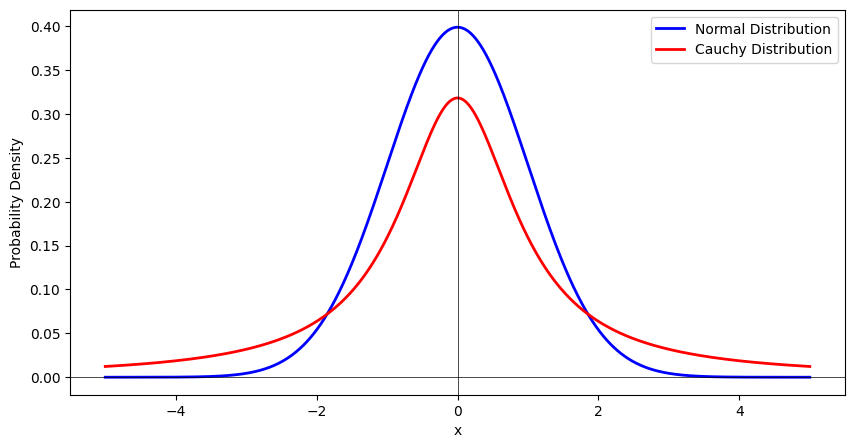
\includegraphics[width=0.9\linewidth]{figures/Gaussian_Cauchy.png}
        \caption{The Student t-distribution with one degree of freedom has heavier tails than the Gaussian.}
    \end{center}
\end{figure}

\section{The Loss Function}
The goal of the algorithm is now to get the similarities $P$ and $Q$ to be as close to each other as possible. 
A common choice for measuring the distance between two distributions is the Kullback-Leibler divergence. 

\begin{defi}[Kullback-Leibler Divergence]
    The \emph{Kullback-Leibler divergence} between two probability distributions $P$ and $Q$ over the same probability space is defined as:
    \[
    D_{\text{KL}}(P \parallel Q) = \sum_{x \in \mathcal{X}} P(x) \log\frac{P(x)}{Q(x)}
    \]
    for discrete distributions where \(\mathcal{X}\) is the domain of the distributions.
\end{defi}

The t-SNE algorithm now aims to find a low-dimensional representation $\mathcal{Y} = (y_1, \dots, y_n)$ that minimizes the KL-divergence between the similarity matrices $P$ and $Q$. 
We thus define the following loss function: 
\begin{equation}
    C(\mathcal{Y}) = D_{\text{KL}}(P \parallel Q) = \sum_{i,j \in \{1,\dots,n\}, i \neq j} p_{ij} \log \frac{p_{ij}}{q_{ij}}
\end{equation}
which leads to the following optimization problem: 
\begin{equation}
    (y_1, \dots y_n) = \argmin_{y_1, \dots y_n} C(\mathcal{Y}) = \argmin_{y_1, \dots y_n} \sum_{i,j \in \{1,\dots,n\}, i \neq j} p_{ij} \log \frac{p_{ij}}{q_{ij}}.
\end{equation}


Note that the Kullback-Leibler divergence is in fact not a metric, since it is not symmetric. 
One can observe that a large $p_{ij}$ being modeled by a small $q_{ij}$ leads to a bigger summand than using a large $q_{ij}$ to model a small $p_{ij}$. 
This means that our loss function places a large cost on using far-apart points to model points that are close in the original dataset. 
On the other hand, there is only a small cost to model points that are actually far apart as nearby in the embedding. 
This shows that we can expect a bigger focus on the preservation of local structure and is important to keep in mind when interpreting t-SNE embeddings, see \cite{Wa16Distill}. 

Notes from \cite{vdMaa14}: In high-dimensional spaces, only small pairwise distances are reliable. This is why most visualization techniques for high-dimensional data only try to model these accurately.

\section{Gradient Descent to Minimize Loss}
Minimizing the cost function can be achieved using a standard gradient-descent type algorithm, with an updating equation of 
\begin{equation}
    y_i^{(k+1)} = y_i^{(k)} + h \frac{\partial C}{\partial y_i}^{(k)} + m^{(k+1)}(y_i^{(k)} - y_i^{(k-1)}) 
\end{equation}
for $i=1,\dots,n$, where $h >0$ is a prespecified step size parameter, $m^{(k)} > 0$ is a momentum parameter and we denote the gradient of our loss function (with respect to $y_i$) as: 
%\begin{equation}
  %  \frac{\partial C}{\partial y_i}^{(k)} = 4 \sum_{1 \leq j \leq n, j \neq i} (y_j^{(k)} - y_i^{(k)}) S_{ij}^{(k)} \in \mathbb{R}^2 \text{ with } S_{ij}^{(k)} = \frac{p_{ij} - q_{ij}^{(k)}}{1+ \norm{y_i^{(k)}-y_j^{(k)}}_2^2 } \in \mathbb{R}
%\end{equation}
\begin{equation}
    \frac{\partial C}{\partial y_i}^{(k)} = 4 \sum_{1 \leq j \leq n, j \neq i} (p_{ij} - q_{ij}^{(k)}) q_{ij}^{(k)} Z^{(k)} (y_j^{(k)} - y_i^{(k)})
\end{equation}
where $Z$ is a global normalization constant: 
\begin{equation}
    Z^{(k)} = \sum_{m \neq l} (1 + \norm{y_m^{(k)} - y_l^{(k)}})^{-1}. 
\end{equation}
\textcolor{red}{\textbf{TO DO}: Check the gradient here, I'm pretty sure it should be $(y_i - y_j)$ and not the other way around}


% algorithm pseudocode here
\begin{algorithm}[H]
    \caption{Basic version of t-Distributed Stochastic Neighbor Embedding}
    \label{alg:tsne}
    \KwIn{data set $\mathcal{X} = \{x_1, x_2, \dots, x_n\}$, perplexity $\text{Perp}$, number of iterations $T$, learning rate $\eta$, momentum $\alpha(t)$}
    \KwOut{Low-dimensional representation $\mathcal{Y}^{(T)} = \{y_1, y_2, \dots, y_n\}$}


    Compute $p_{ij}$ with perplexity $\text{Perp}$ 
    
    Sample initial solution $\mathcal{Y}^{(0)} = \{y_1, y_2, \dots, y_n\} \sim \mathcal{N}(0, 10^{-4} I)$\

    \For{$t = 1$ \KwTo $T$}{
        Compute low-dimensional affinities $q_{ij}$ 

        Compute gradient $\frac{\delta C}{\delta \mathcal{Y}}$ 

        Update solution:

        \[
        \mathcal{Y}^{(t)} = \mathcal{Y}^{(t-1)} + \eta \frac{\delta C}{\delta \mathcal{Y}} + \alpha(t) (\mathcal{Y}^{(t-1)} - \mathcal{Y}^{(t-2)})
        \]
    }

    \Return $\mathcal{Y}^{(T)}$\
\end{algorithm}
\textcolor{red}{\textbf{TO DO}: make algorithm look nicer}

To optimize the gradient descent prodcedure, \cite{vdMaa08} proposes the following: 
\begin{itemize}
    \item setting the momentum term to $\alpha^{(t)} = 0.5$ for $t<250$ and $\alpha^{(t)} = 0.8$ for $t \geq 250$
    \item set intial learning rate to $\eta = 100$ and update after every iteration adaptively using the adaptive learning rate scheme described by Jacobs \cite{Jacobs1988}
\end{itemize}


